\documentclass[12pt]{article}
\usepackage[brazil]{babel}
\usepackage[utf8]{inputenc}
\usepackage{amsmath}
\usepackage{amsfonts}
\usepackage{amssymb}
\usepackage{geometry}
\usepackage{graphicx}
\usepackage{float}
\usepackage{enumitem}
\usepackage{multicol}
\usepackage{array}
\usepackage{xcolor}
\usepackage[T1]{fontenc}

\newif\ifmostravermelho
%\mostravermelhofalse %começa falso

\newcommand{\vermelho}[1]{%
  \ifmostravermelho
    {\color{red}#1}%
  \else
    #1%
  \fi
}

%\newcommand{\vermelho}[1]{{\color{red}#1}}
\geometry{a4paper, margin=1.2cm}
\setlength{\parindent}{1.2cm}

% implementa contador
% Definindo o contador e o comando de questão
\newcounter{questao}
\newcommand{\novaquestao}[1]{%
  \stepcounter{questao}%
  \subsection*{Questão \thequestao\ (#1)}%
}

\begin{document}
    % Cabeçalho reduzido
    \vspace{0.5cm}
    \begin{center}
        \large
        \begin{tabular}{|l l|}
            \hline
            \textbf{ESCOLA:} & EETI GILBERTO MESTRINHO DE MEDEIROS RAPOSO \\ 
            \textbf{ALUNA(O):} & \underline{\hspace{7cm}} \textbf{SÉRIE:} \underline{\hspace{1.5cm}} \textbf{TURMA:} \underline{\hspace{1.5cm}} \\
            \textbf{PROFESSOR:} & \underline{\hspace{7cm}} \textbf{DATA:} \underline{\hspace{1.5cm}}/\underline{\hspace{1.5cm}}/\underline{\hspace{1.5cm}} \\
            \textbf{VALOR:} & \underline{\hspace{3cm}} \textbf{NOTA:} \underline{\hspace{1.5cm}} \\
            \hline
        \end{tabular}
    \end{center}
    \vspace{0.5cm}
    
    % Título manual
    \begin{center}
        \Large\textbf{LISTA DE EXERCÍCIOS SOBRE PROGRESSÃO ARITMÉTICA (P.A) E PROGRESSÃO GEOMÉTRICA (P.G)}
    \end{center}
    
    \vspace{0.3cm}
    
    \section*{\vermelho{ATENÇÃO:}}
    \begin{itemize}[noitemsep]
        \item Resolva toda a lista, justificando cada questão.
        \item Colocar o nome completo e identificação no cabeçalho.
        \item Faça na lista, se e somente se a resolução de cada questão couber em cada questão.
        \item Há apenas uma opção correta em cada questão de múltipla escolha.
        \item Caso opte por fazer numa folha à parte, identifique cada questão. \\
    \end{itemize}
    % Início das colunas com linha vertical
    %\mostravermelhotrue
    \begin{multicols}{2}
        \columnseprule=0.4pt
        \columnsep=20pt
        
        \novaquestao{MACRO UEA - 2013}
            A previsão é iniciar as operações em setembro de 2016 e atingir a capacidade total de produção em setembro de 2018. Admita que três números indiquem, no cronograma, a capacidade de produção (em milhões de toneladas) em três momentos distintos desse processo, e que esses três números estejam em Progressão Aritmética crescente de razão 15. Se subtrairmos 9 do termo central, os números passam a formar uma Progressão Geométrica. A capacidade de produção prevista no cronograma para o terceiro momento é, em milhões de toneladas, igual a:
            
            \begin{enumerate}[label=(\alph*), noitemsep]
                \item $32$
                \item $17$
                \item $22$
                \item $34$
                \item $28$
            \end{enumerate}
        
        \novaquestao{SIS UEA - 2023}
            Em uma progressão aritmética com 30 termos, a soma dos 2 maiores termos é 139. Sabendo que a razão dessa progressão é 3, a soma dos seus 2 menores termos é:
        
            \begin{enumerate}[label=(\alph*), noitemsep]
                \item $-29$
                \item $-10$
                \item $0$
                \item $23$
                \item $49$
            \end{enumerate}
        
        \novaquestao{PSC UFAM - 2003}
            As medidas das arestas de um paralelepípedo retângulo formam uma P.G.. Se a menor das arestas mede $ 0,3 \ cm$ e o volume de tal paralelepipedo é $27\ cm^{3}$. Então, a soma das áreas de suas faces é:
            
            \begin{enumerate}[label=(\alph*), noitemsep]
                \item $99,9\ cm^{2}$
                \item $90\ cm^{2}$
                \item $199,8\ cm^{2}$
                \item $90,9\ cm^{2}$
                \item $209,9\ cm^{2}$
            \end{enumerate}
        
        \novaquestao{ENEM - 2014}
        
            Um ciclista participará de uma competição e treinará alguns dias da seguinte maneira: no primeiro dia, pedalará 60 km; no segundo dia, a mesma distância do primeiro mais r km; no terceiro dia, a mesma distância do segundo mais r km; e, assim, sucessivamente, sempre pedalando a mesma distância do dia anterior mais r km. No último dia, ele deverá percorrer 180 km, completando o treinamento com um total de 1 560 km. A distância r que o ciclista deverá pedalar a mais a cada dia, em km, é:

            \begin{enumerate}[label=(\alph*), noitemsep]
                \item $3$
                \item $7$
                \item $10$
                \item $13$
                \item $20$
            \end{enumerate}
        
        \novaquestao{MACRO UEA - 2023}
            O salário de determinado estagiário em uma empresa, em janeiro, era de $R\$ 1.500,00$. Esse salário teve um acréscimo mensal constante, sempre sobre o valor recebido no mês anterior, durante os meses de fevereiro, março, abril e maio. Se o salário no mês de maio foi de $R\$ 5.000,00$, o salário no mês de abril foi de:

            \begin{enumerate}[label=(\alph*), noitemsep]
                \item $R\$ 3.250,00.$
                \item $R\$ 4.575,00.$
                \item $R\$ 4.125,00.$
                \item $R\$ 2.375,00.$               
                \item $R\$ 2.950,00.$

            \end{enumerate}
        
        \novaquestao{MACRO UEA - 2023}
            As notas de matemática obtidas por um estudante na 1\textordfeminine, \ 2\textordfeminine \ e \ 3\textordfeminine \ provas do ano formam, nessa ordem, uma progressão aritmética de razão 3. Se o estudante tivesse obtido um ponto a mais na 1\textordfeminine \ prova e mantivesse as mesmas notas da 2\textordfeminine \  e \ da 3\textordfeminine \ provas, essa nova sequência de notas, nessa ordem, formaria uma progressão geométrica de razão 3/2 . A nota obtida por ele na 3\textordfeminine \  prova foi:

        
            \begin{enumerate}[label=(\alph*), noitemsep]
                \item $6$
                \item $9$
                \item $8$
                \item $7$
                \item $10$
            \end{enumerate}
        
        \novaquestao{MACRO UEA - 2021}
            Uma pessoa possui em sua carteira somente moedas de $R\$\ 0,25$, de $R\$\ 0,50$ e de $R\$\ 1,00$, no total de 18 moedas. O número de moedas de $R\$\ 0,25$, de $R\$\ 0,50$ e de $R\$\ 1,00$ forma, nesta ordem, uma progressão aritmética de razão $-2$. Todas essas moedas juntas totalizam o valor de:
            
            \begin{enumerate}[label=(\alph*), noitemsep]
                \item $R\$ \ 12,00.$
                \item $R\$ \ 9,00.$
                \item $R\$ \ 11,00.$
                \item $R\$ \ 10,00.$
                \item $R\$ \ 13,00.$
            \end{enumerate}
        
        \novaquestao{ENEM - 2016}
        
            Sob a orientação de um mestre de obras, João e Pedro trabalharam na reforma de um edifício. João efetuou reparos na parte hidráulica nos andares 1, 3, 5, 7, e assim sucessivamente, de dois em dois andares. Pedro trabalhou na parte elétrica nos andares 1,4, 7, 10, e assim sucessivamente, de três em três andares. Coincidentemente, terminaram seus trabalhos no último andar. Na conclusão da reforma, o mestre de obras informou, em seu relatório, o número de andares do edifício. 
            Sabe-se que, ao longo da execução da obra, em exatamente 20 andares, foram realizados reparos nas partes hidráulica e elétrica por João e Pedro.  Qual é o número de andares desse edifício?
        
            \begin{enumerate}[label=(\alph*), noitemsep]
                \item $2018$
                \item $2023$
                \item $2031$
                \item $2035$
                \item $2043$
            \end{enumerate}
        
        \novaquestao{MACRO UEA - 2021}
            Na progressão aritmética (a, 11, b, c, 20), os valores de a e c correspondem, respectivamente, às medidas, em centímetros, de um cateto e da hipotenusa de um triângulo retângulo. O valor do outro cateto desse triângulo é igual a:
        
            \begin{enumerate}[label=(\alph*), noitemsep]
                \item $9 \ cm$
                \item $17 \ cm$
                \item $5 \ cm$
                \item $15 \ cm$
                \item $12 \ cm$
            \end{enumerate}
        
        \novaquestao{MACRO UEA - 2021}
            Uma pessoa comprou abacaxis, mangas e laranjas de modo que o número de unidades compradas de cada tipo de fruta, nesta ordem, formava uma progressão geométrica de razão 2. Sabendo que a diferença entre o número de laranjas e o número de abacaxis foi 9, o número total de frutas compradas foi:
        
            \begin{enumerate}[label=(\alph*), noitemsep]
                \item $24$
                \item $27$
                \item $21$
                \item $18$
                \item $30$
            \end{enumerate}
        
        \novaquestao{MACRO UEA - 2012}
        
            Uma cervejaria artesanal, com sede em Belém, pretende exportar seus produtos já no início de 2013. A intenção é surpreender o mercado internacional com uma mistura de malte e frutas típicas da região. Para tanto, elaborou uma previsão na qual as quantidades de litros que serão exportados a cada mês estão em progressão aritmética (PA) crescente. 
            Sabe-se que a soma do primeiro (janeiro) e quarto (abril) termos dessa PA é igual a $53.200$ litros. Se a razão da PA é igual a $60\%$ do primeiro termo, então a quantidade de litros prevista para ser exportada em março é:
        
            \begin{enumerate}[label=(\alph*), noitemsep]
                \item $24.200$
                \item $34.200$
                \item $32.600$
                \item $30.800$
                \item $22.400$
            \end{enumerate}
        
        \novaquestao{MACRO UEA - 2020}
            Um grupo de amigos foi a uma cafeteria e, juntos, gastaram $R\$ 180,00$. Cada um deles pagou seu próprio consumo, sendo $R\$ 24,00$ o menor valor e $R\$ 48,00$ o maior. Sabendo que os valores pagos por esse grupo de amigos formavam uma progressão aritmética, o número de amigos desse grupo era:        
        
            \begin{enumerate}[label=\alph*), noitemsep]
                \item $7$
                \item $3$
                \item $5$
                \item $4$
                \item $6$
            \end{enumerate}
        
        \novaquestao{MACRO UEA - 2020}
            Em um laboratório, há 3 frascos com o mesmo tipo de produto, cujas quantidades, todas diferentes entre si, formam uma progressão geométrica de razão 4. Se a soma das 3 quantidades totaliza 315 mL, a menor quantidade de produto contida em um frasco é:
        
            \begin{enumerate}[label=(\alph*), noitemsep]
                \item $25\ mL$
                \item $20\ mL$
                \item $30\ ml$
                \item $15\ ml$
                \item $10\ ml$
            \end{enumerate}

        \novaquestao{MACRO UEA - 2020}
        
            Para a realização de determinada tarefa foram cortados 4 pedaços de barbante, P1, P2, P3 e P4, cujos comprimentos formam, nesta ordem, uma progressão geométrica crescente. Se o menor pedaço mede 40 cm e a diferença entre os comprimentos dos pedaços P2 e P1 é 20 cm, o comprimento do maior pedaço excede o comprimento do menor pedaço em:

            \begin{enumerate}[label=(\alph*), noitemsep]
                \item $95\ cm$
                \item $65\ cm$
                \item $75\ cm$
                \item $85\ cm$
                \item $55\ cm$
            \end{enumerate}

        \novaquestao{MACRO UEA - 2019}
            Em negociação com o lojista, Clarice obteve um desconto de $10\%$ sobre o preço original P de certo produto, obtendo o preço P1. Ela continuou a negociação e obteve mais $10\%$ de desconto sobre P1, obtendo o preço final P2. Se P2  é igual a $R\$\ 1.215,00$, então o preço original P era igual a:

            \begin{enumerate}[label=(\alph*), noitemsep]
                \item $R\$\ 1.350,00$
                \item $R\$\ 1.550,00$
                \item $R\$\ 1.500,00$
                \item $R\$\ 1.400,00$
                \item $R\$\ 1.450,00$
            \end{enumerate}

        \novaquestao{ENEM - 2020}
            No Brasil, o tempo necessário para um estudante realizar sua formação até a diplomação em um curso superior, considerando os 9 anos de ensino fundamental, os 3 anos do ensino médio e os 4 anos de graduação (tempo médio), é de 16 anos. No entanto, a realidade dos brasileiros mostra que o tempo médio de estudo de pessoas acima de 14 anos é ainda muito pequeno, conforme apresentado na tabela.

            \begin{center}
                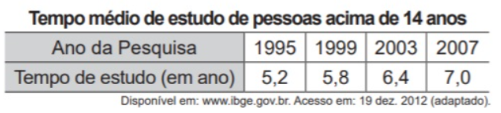
\includegraphics[scale=0.5]{q16.png}
            \end{center}Considere que o incremento no tempo de estudo, a cada período, para essas pessoas, se mantenha constante até o ano 2050, e que se pretenda chegar ao patamar de $70\%$ do tempo necessário à obtenção do curso superior dado anteriormente. O ano em que o tempo médio de estudo de pessoas acima de 14 anos atingirá o percentual pretendido será:

            \begin{enumerate}[label=(\alph*), noitemsep]
                \item $2018$
                \item $2023$
                \item $2031$
                \item $2035$
                \item $2043$
            \end{enumerate}

        \novaquestao{MACRO UEA - 2019}
            Um lojista abriu sua primeira loja. Dois anos depois, inaugurou sua segunda loja e, dois anos após essa inauguração, abriu sua terceira loja, procedendo sempre da mesma maneira até chegar à oitava e última loja. Ou seja, todas as lojas foram inauguradas observando-se sempre o mesmo intervalo de tempo, de exatos dois anos, entre cada inauguração. Hoje, o tempo de atividade da primeira loja é igual ao quíntuplo do tempo de atividade da oitava loja. Desse modo, hoje, o tempo de atividade da oitava loja é de:

            \begin{enumerate}[label=(\alph*), noitemsep]
                \item 2 anos
                \item 2,5 anos
                \item 3,5 anos
                \item 4 anos
                \item 3 anos
            \end{enumerate}

        \novaquestao{MACRO UEA - 2019}
            As massas, em quilogramas, de três blocos constituem uma progressão geométrica de razão positiva, cujo primeiro termo é 3. Sabendo-se que a média aritmética dos três termos é 21, a massa do bloco que corresponde ao terceiro termo dessa progressão é:

            \begin{enumerate}[label=(\alph*), noitemsep]
                \item 32 kg
                \item 36 kg
                \item 48 kg
                \item 63 kg
                \item 27 kg
            \end{enumerate}

        \novaquestao{MACRO UEA - 2018}
        
            Um casal tem cinco filhos cujas idades, em anos, formam uma progressão aritmética decrescente de razão $r$. Sabe-se que, hoje, a idade do filho mais novo é igual a $-2r$ e que a idade do filho mais velho é igual ao triplo da idade do filho mais novo. Se, hoje, a soma das idades dos cinco filhos é igual a 60 anos, o nascimento do filho mais velho ocorreu em:
        
    
            \begin{enumerate}[label=(\alph*), noitemsep]
                \item 1996
                \item 1998
                \item 2000
                \item 2002
                \item 1994
            \end{enumerate}

        \novaquestao{ENEM - 2023}
            O gerente de uma fábrica pretende comparar a evolução das vendas de dois produtos similares (I e II). Para isso, passou a verificar o número de unidades vendidas de cada um desses produtos em cada mês. Os resultados dessa verificação, para os meses de abril a junho, são apresentados na tabela. 
            \begin{center}
                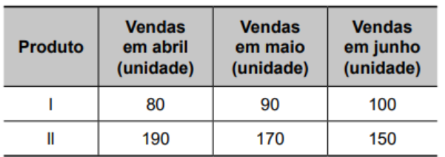
\includegraphics[scale=0.6]{q20.png}
            \end{center}O gerente estava decidido a cessar a produção do produto II no mês seguinte àquele em que as vendas do produto I superassem as do produto II. Suponha que a variação na quantidade de unidades vendidas dos produtos I e II se manteve, mês a mês, como no período representado na tabela. Em qual mês o produto II parou de ser produzido?

            
            \begin{enumerate}[label=(\alph*), noitemsep]
                \item Junho
                \item Julho
                \item Agosto
                \item Setembro
                \item Outubro
            \end{enumerate}

        \novaquestao{MACRO UEA - 2018}
            Impulsionado pela Copa do Mundo, um grande varejista elaborou uma previsão de vendas de televisores para o primeiro semestre de 2018, na qual os números de unidades a serem vendidas a cada mês constituíam uma progressão aritmética crescente. Sabe-se que para janeiro estavam previstas $3.500$ unidades e que $60\%$ do número de unidades previstas para o bimestre março/abril correspondia a $7.200$ unidades. De acordo com a previsão, o número de unidades a serem vendidas de janeiro até maio era igual a:

            \begin{enumerate}[label=(\alph*), noitemsep]
                \item $25.500$
                \item $27.500$
                \item $26.000$
                \item $27.000$
                \item $24.000$
            \end{enumerate}

            \novaquestao{MACRO UEA - 2016}

                Daniel emprestou $R\$\ 21.250,00$ a seu amigo Leonardo. O pagamento do valor total emprestado, sem o acréscimo de juros, será feito em uma sequência de 10 parcelas mensais, na qual os valores das parcelas constituem uma progressão aritmética crescente de razão r. Se o valor da primeira parcela é $R\$\ 1.000,00$, a soma dos valores da oitava, nona e décima parcelas é igual a:
            
                \begin{enumerate}[label=(\alph*), noitemsep]
                    \item $R\$\ 8.250,00$
                    \item $R\$\ 9.000,00$
                    \item $R\$\ 8.750,00$
                    \item $R\$\ 7.800,00$
                    \item $R\$\ 8.600,00$
                \end{enumerate}

        \novaquestao{MACRO UEA - 2016}
        
            Em uma progressão aritmética crescente, a soma do primeiro e do quarto termos é 210. Se a razão é igual a ${1}/{2}$ do primeiro termo, então o quinto termo dessa progressão é:
        
            \begin{enumerate}[label=(\alph*), noitemsep]
                \item 160
                \item 140
                \item 120
                \item 150
                \item 180
            \end{enumerate}

        \novaquestao{ENEM - 2018}

            A prefeitura de um pequeno município do interior decide colocar postes para iluminação ao longo de uma estrada retilínea, que inicia em uma praça central e termina numa fazenda na zona rural. Como a praça já possui iluminação, o primeiro poste será colocado a 80 metros da praça, o segundo, a 100 metros, o terceiro, a 120 metros, e assim sucessivamente, mantendo-se sempre uma distância de vinte metros entre os postes, até que o último poste seja colocado a uma distância de $1.380$ metros da praça. Se a prefeitura pode pagar, no máximo, $R\$\ 8.000,00$ por poste colocado, o maior valor que poderá gastar com a colocação desses postes é

        
            \begin{enumerate}[label=(\alph*), noitemsep]
                \item $R\$\ 512.000,00$
                \item $R\$\ 520.000,00$
                \item $R\$\ 528.000,00$
                \item $R\$\ 552.000,00$
                \item $R\$\ 584.000,00$
            \end{enumerate}

        \novaquestao{MACRO UEA - 2015}
            Em uma progressão geométrica de 10 termos, temos $S_{3}= -9$ e $S_{4}= 15$, que são, respectivamente, as somas dos três primeiros e dos quatro primeiros termos da sequência. Se o termo inicial é $-3$, o décimo termo dessa progressão é igual a
        
            \begin{enumerate}[label=(\alph*), noitemsep]
                \item $-1536$
                \item $-768$
                \item $3072$
                \item $768$
                \item $1536$
            \end{enumerate}

        \novaquestao{MACRO UEA - 2014}
            Os números que indicam a quantidade de barcos utilizados por certa empresa de turismo em 2011, 2012 e 2013 estão em progressão geométrica crescente. Sabe-se que a soma desses três números é 28 e que, em 2012, a empresa utilizou 8 barcos. Desse modo, o número de barcos que essa empresa utilizou em 2013 foi:

            \begin{enumerate}[label=(\alph*), noitemsep]
                \item 16
                \item 24
                \item 12
                \item 32
                \item 10 
            \end{enumerate}
        

        \novaquestao{ ENEM - 2024}
            Um novo condomínio foi construído na Rua X. Alguns lotes já receberam numeração da prefeitura, enquanto outros apresentam apenas o sobrenome do seu proprietário. O servidor da prefeitura numerará os lotes que ainda não foram numerados. Para isso, ele observa o padrão da numeração já existente, conforme apresentado na figura, percebendo que, em cada lado da rua, as sequências das numerações formam progressões aritméticas, e, com isso, atribui um número ao lote da família Costa.

            \begin{center}
                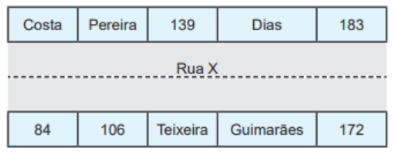
\includegraphics[scale=0.6]{q27.png}
            \end{center}O número atribuído ao lote da família Costa é:
        
            \begin{enumerate}[label=(\alph*), noitemsep]
                \item 51
                \item 73
                \item 95
                \item 117
                \item 161
            \end{enumerate}

        \novaquestao{MACRO UEA - 2013}
            Observe as informações.
            
            \begin{center}
                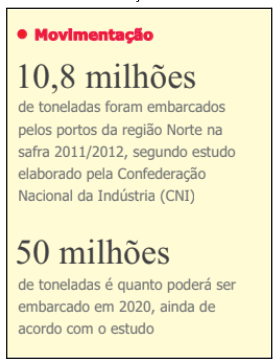
\includegraphics[scale=0.7]{q28.png}
            \end{center}Admita que, na previsão elaborada pela CNI, os números que indicam as toneladas de grãos embarcadas anualmente estejam em Progressão Aritmética crescente de razão r, na qual o primeiro termo é o número de toneladas embarcadas em 2012, e o último, o número de toneladas previstas para 2020. Nessas condições, prevê-se que a quantidade total de grãos embarcados, de 2012 a 2020, será, em milhões de toneladas, igual a:
            
            \begin{enumerate}[label=(\alph*), noitemsep]
                \item $254,6$
                \item $273,6$
                \item $290,2$
                \item $268,4$
                \item $243,2$
            \end{enumerate}

        \novaquestao{MACRO UEA - 2012}
            Um grupo de amigos apostou 50 reais no concurso de números 395 de certa loteria. A partir daí, o valor apostado em cada um dos concursos seguintes cresceu em progressão aritmética de razão 6, até que atingiu o valor máximo de 170 reais. Sabendo que o grupo apostou em todos os concursos seguintes ao de número 395, sem exceção, pode-se afirmar que o valor de 170 reais foi apostado no concurso de número:

            \begin{enumerate}[label=(\alph*), noitemsep]
                \item 412
                \item 413
                \item 410
                \item 416
                \item 415
            \end{enumerate}

        \novaquestao{ENEM - 2024}
            É comum pensarmos na equivalência entre a idade de um animal de estimação, no caso de cães e gatos, e de um ser humano. De acordo com as diretrizes de idade criadas pela American Animal Hospital Association (AAHA), o International Cat Care e a American Association of Feline Practitioners (AAFP), a última fase da vida de um gato é chamada de geriátrica e começa aos 15 anos de vida do animal. A tabela apresenta os primeiros anos da fase geriátrica da equivalência entre a idade do gato e a idade de um humano. Sabe-se que o gato mais velho do mundo morreu ao completar 38 anos de vida. Considere que o padrão observado na tabela se mantém.
            
            \begin{center}
                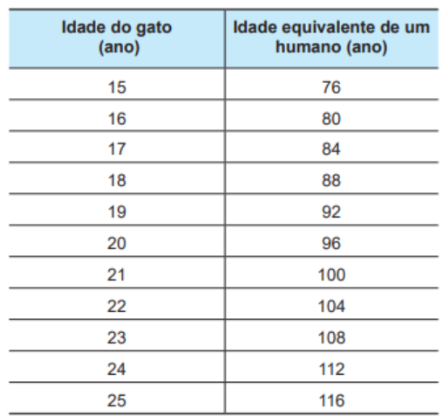
\includegraphics[scale=0.6]{q30.png}
            \end{center}De acordo com os dados apresentados, a idade em que o gato mais velho do mundo morreu é equivalente a qual idade, em ano, de um humano?

            \begin{enumerate}[label=(\alph*), noitemsep]
                \item 129
                \item 133
                \item 158
                \item 168
                \item 176
            \end{enumerate}

        \novaquestao{Unicamp 2020}
            Considere que (a,b,3,c) é uma progressão aritmética de números reais, e que a soma de seus elementos é igual a 8. O produto dos elementos dessa progressão é igual a:

            \begin{enumerate}[label=(\alph*), noitemsep]
                \item $30$
                \item $10$
                \item \vermelho{$-15$} %
                \item $-20$
                \item $-25$
            \end{enumerate}

        \novaquestao{Ciaba 2004}

             Dada uma progressão aritmética, em que o quinto elemento é 17 e o terceiro é 11, calcule a soma dos sete primeiros termos dessa progressão aritmética:

            \begin{enumerate}[label=(\alph*), noitemsep]
                \item 90
                \item 92
                \item 94 
                \item 96
                \item \vermelho{98}
            \end{enumerate}

        \novaquestao{UFMS 2022}
            Seja (a,b,c) uma progressão geométrica de números reais. Suponha que $a+b+c=26$ e $a^{2}+b^{2}+c^{2}=364$. Nessas condições, qual o valor de b? 

            \begin{enumerate}[label=(\alph*), noitemsep]
                \item 4
                \item 6 
                \item 8
                \item 10 
                \item 12
            \end{enumerate}
        
        \novaquestao{Enem Libras - 2018}
            A figura ilustra uma sequência de formas geométricas formadas por palitos, segundo uma certa regra.

            \begin{center}
                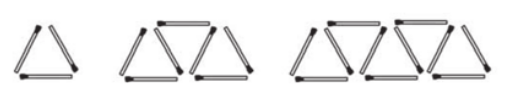
\includegraphics[scale=0.5]{q34.png}
            \end{center}Continuando a sequência, segundo essa mesma regra, quantos palitos serão necessários para construir o décimo termo da sequência?

            \begin{enumerate}[label=(\alph*), noitemsep]
                \item 30
                \item 39
                \item 40
                \item 43
                \item 57
            \end{enumerate}

        \novaquestao{Unesp 2017}
            A figura indica o empilhamento de três cadeiras idênticas e perfeitamente encaixadas umas nas outras, sendo h a altura da pilha em relação ao chão.

            \begin{center}
                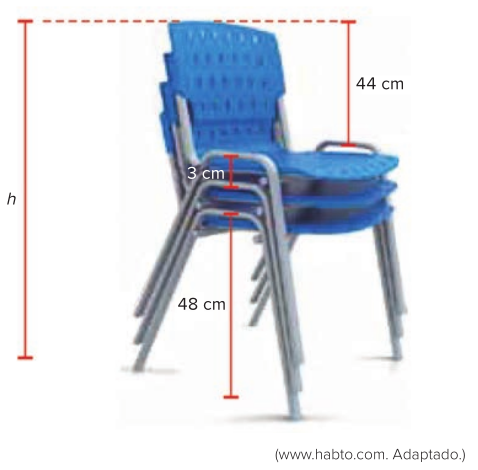
\includegraphics[scale=0.5]{q35.png}
            \end{center} A altura, em relação ao chão, de uma pilha de \textit{n} cadeiras perfeitamente encaixadas umas nas outras, será igual a $1,4$ m se \textit{n} for igual a:
        
            \begin{enumerate}[label=(\alph*), noitemsep]
                \item \vermelho{$30$} % 
                \item $60$ 
                \item $15$  
                \item $45$  
                \item $50$
            \end{enumerate}

        \novaquestao{UPF-RS - 2021}
            Um supermercado pretende fazer a promoção de um determinado produto colocando uma pilha de latas desse produto de modo que cada linha tenha menos uma lata do que a anterior. No local onde será colocada a pilha de latas há disponibilidade de 2 m para a altura dessa pilha. A pilha termina com apenas uma lata, como mostra a figura, e cada lata tem 10 cm de altura. O número de latas que serão utilizadas para construir essa pilha é:

            \begin{center}
                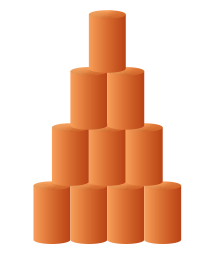
\includegraphics[scale=0.6]{q36.png}
            \end{center}
        
            \begin{enumerate}[label=(\alph*), noitemsep]
                \item 420
                \item 200
                \item 110
                \item 20
                \item 210
            \end{enumerate}

        \novaquestao{Escola Naval-RJ 2015}
            A soma dos três primeiros termos de uma PG crescente vale 13 e a soma dos seus quadrados 91. Justapondo-se esses termos, obtém-se um número de três algarismos. Pode-se afirmar que o resto da divisão desse número pelo inteiro 23 vale:

            \begin{enumerate}[label=(\alph*), noitemsep]
                \item 1
                \item 4
                \item 8
                \item 9
                \item 11
            \end{enumerate}
        
        \novaquestao{ExPCEx-SP 2022}
            O Cap R. Gomes é um autêntico “canga”, isto é, um militar que não apenas coopera com os membros de sua equipe, mas estimula superiores, pares e subordinados ao bom cumprimento das missões. Em particular, ele incentiva um grupo de militares a melhorar o desempenho na corrida. Para tal, criou um programa de treinamento em que é preciso correr exatamente 576 km no total, começando com 26 km na primeira semana e, a partir da segunda, acrescentando exatos 4 km a cada semana, ou seja, cada integrante do grupo deve correr exatamente 26 km na 1\textordfeminine\ semana, 30 km na 2\textordfeminine\  semana, 34 km na 3\textordfeminine\ semana e assim sucessivamente. Após quantas semanas a meta de 576 km será atingida?

            
            \begin{enumerate}[label=(\alph*), noitemsep]
                \item 10
                \item 11
                \item 12
                \item 13
                \item 14
            \end{enumerate}

        \novaquestao{Poliedro-SP}
            Considere a seguinte sequência infinita de sólidos geométricos.

            \begin{center}
                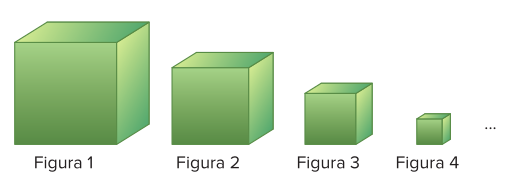
\includegraphics[scale=0.5]{q39.png}
            \end{center}Cada um desses sólidos é um cubo, e cada cubo, a partir do segundo, tem medida de aresta igual à metade da medida da aresta do cubo da figura anterior. Sendo L a medida da aresta do cubo da Figura 1, qual é o volume total de todos os cubos dessa sequência?

            \begin{enumerate}[label=(\alph*), noitemsep]
                \item $L^{3}$ \\
                \item $\dfrac{8}{7}L^{3}$ \\
                \item $\dfrac{73}{64}L^{3}$ \\ 
                \item $\dfrac{585}{512}L^{3}$ \\
                \item $2L^{3}$
            \end{enumerate}

        \novaquestao{ENEM 2018}
            Um quebra-cabeça consiste em recobrir um quadrado com triângulos retângulos isósceles, como ilustra a figura.

            \begin{center}
                
\includegraphics[scale=0.6]{q40.png}
            \end{center}Uma artesã confecciona um quebra-cabeça como o descrito, de tal modo que a menor das peças é um triângulo retângulo isósceles cujos catetos medem 2 cm. O quebra-cabeça, quando montado, resultará em um quadrado cuja medida do lado, em centímetro, é
            
            \begin{enumerate}[label=(\alph*), noitemsep]
                \item 14
                \item 12
                \item $7\sqrt{2}$ 
                \item $6+4\sqrt{2}$
                \item $6+2\sqrt{2}$ 
            \end{enumerate}
        
            
    \end{multicols}
    
\end{document}